\documentclass[landscape]{article}
\usepackage[a4paper,landscape,margin=1.5cm]{geometry}
\usepackage{graphicx}
\usepackage{array}
\usepackage{tabularx}
\usepackage{colortbl}
\usepackage{xcolor}
\usepackage{fancyhdr}
\usepackage{tikz}
\usepackage{booktabs}
\usepackage{subcaption}
\usepackage{pagecolor}

\graphicspath{{illustration/}{reference/}}  % DO NOT CHANGE THIS LINE

% Define custom colors
\definecolor{headergreen}{RGB}{0,100,0} % Dark green color
\definecolor{lightgray}{RGB}{240,240,240}
\definecolor{lightbeige}{RGB}{252,250,245} % Light beige color
\pagecolor{lightbeige} % Set background color

% Custom page style
\pagestyle{fancy}
\fancyhf{}
\renewcommand{\headrulewidth}{0pt}
\cfoot{\textcolor{headergreen}{\thepage}} % Added page number in footer center

\begin{document}
% Header Section
\begin{center}
\Huge\bfseries\sffamily\textcolor{headergreen}{TECHNICAL SPECIFICATION SHEET}
\end{center}

\vspace{0.5cm}

% PRODUCT DETAILS
\noindent\begin{tabularx}{\textwidth}{|X|X|X|X|}
\hline
\rowcolor{headergreen}\multicolumn{4}{|c|}{\textcolor{white}{\textbf{PRODUCT DETAILS}}} \\
\hline
Brand Name: W & Designer: E & Season: Autumn/Winter & Category: Outerwear \\
\hline
Date: March 2025 & Style Name: Elegant Dark Green Coat & Style Number: 002 & Main Fabric: Wool \\
\hline
\end{tabularx}

\vspace{0.5cm}

% STYLE DESCRIPTION
\noindent\begin{tabularx}{\textwidth}{|X|}
\hline
\rowcolor{headergreen}\multicolumn{1}{|c|}{\textcolor{white}{\textbf{STYLE DESCRIPTION}}} \\
\hline
An elegant dark green coat featuring a tailored fit with clean lines, designed for a sophisticated look. The coat is crafted from high-quality wool, offering warmth and comfort, perfect for the cooler months.
\end{tabularx}
\hline

\vspace{0.5cm}

% TECHNICAL DRAWINGS
\noindent\begin{tabularx}{\textwidth}{|X|}
\hline
\rowcolor{headergreen}\multicolumn{1}{|c|}{\textcolor{white}{\textbf{TECHNICAL DRAWINGS}}} \\
\hline
\begin{center}
% First row of drawings
\begin{tabular}{c}
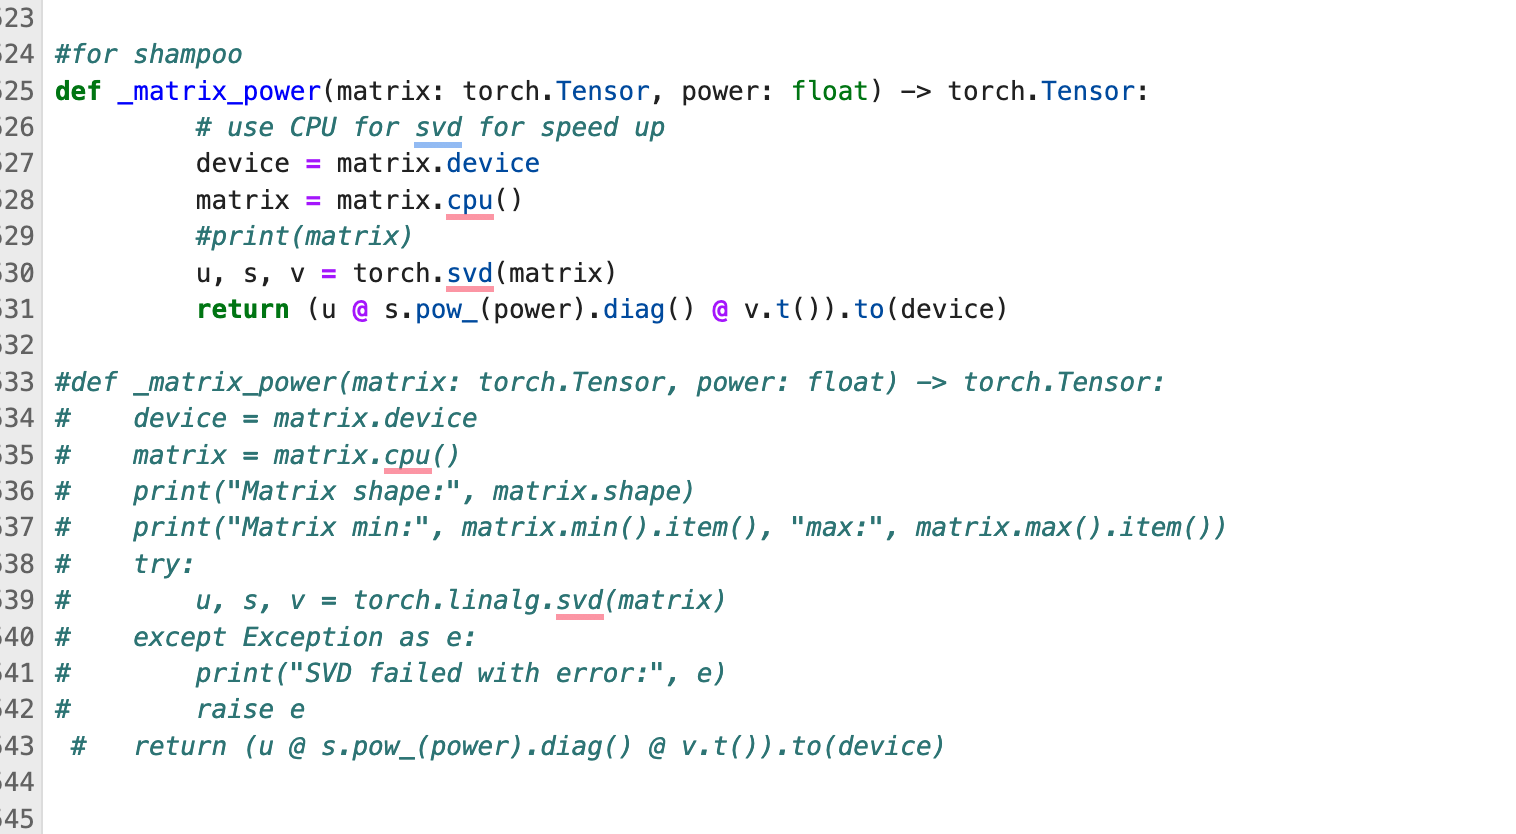
\includegraphics[width=0.4\textwidth,height=8cm,keepaspectratio]{Screenshot_2025-03-09_at_15.26.02.png} \\
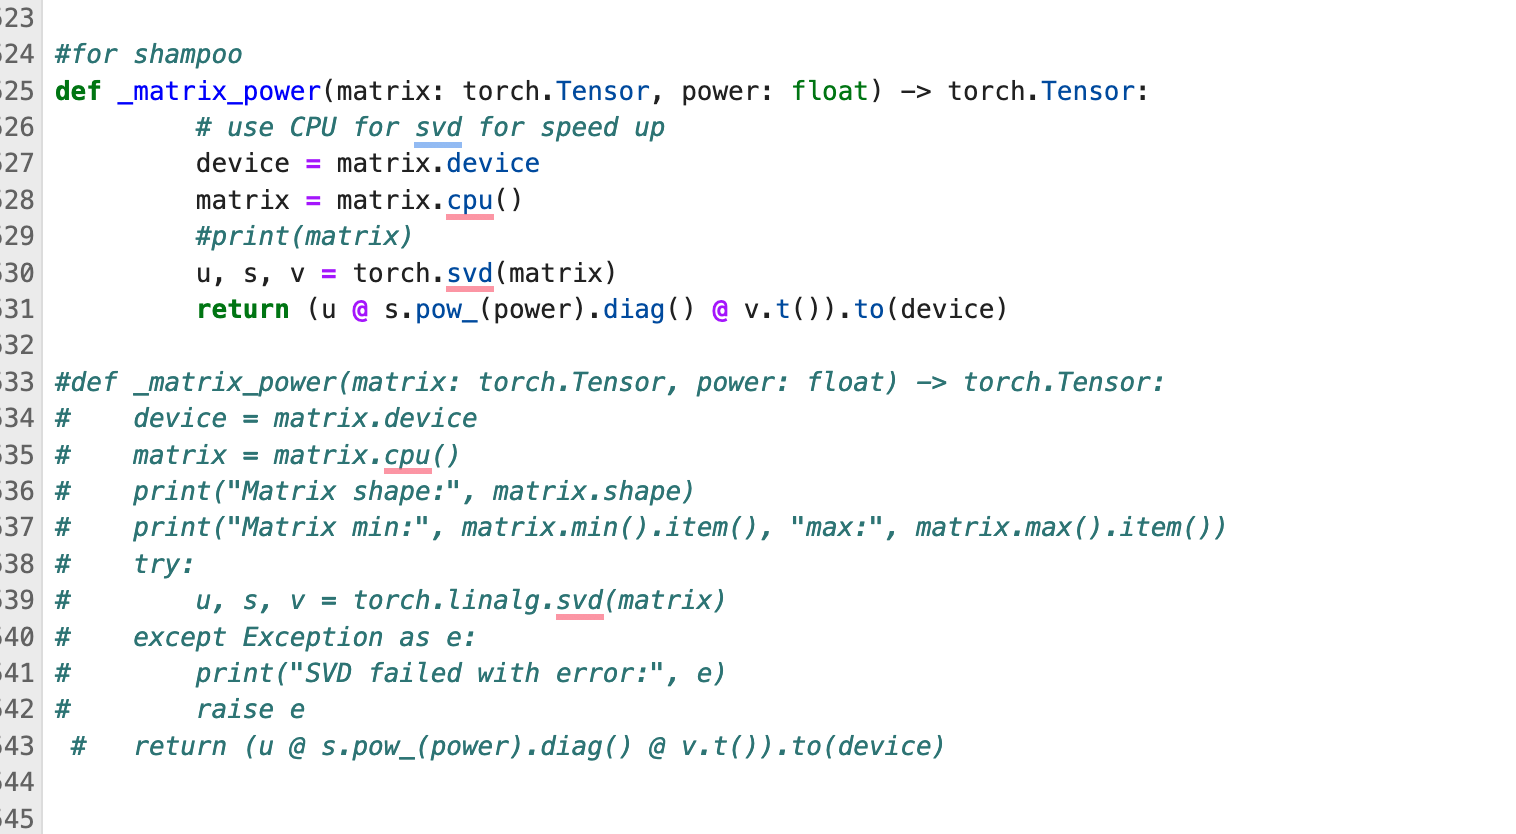
\includegraphics[width=0.4\textwidth,height=8cm,keepaspectratio]{Screenshot_2025-03-09_at_15.26.02.png} \\
\end{tabular}
\end{center}
\end{tabularx}
\hline

\vspace{0.5cm}

\newpage
% MEASUREMENTS
\noindent\begin{tabularx}{\textwidth}{|X|X|X|X|X|X|X|}
\hline
\rowcolor{headergreen}\multicolumn{7}{|c|}{\textcolor{white}{\textbf{MEASUREMENTS}}} \\
\hline
\textbf{Item} & \textbf{Description} & \textbf{XS} & \textbf{S} & \textbf{M} & \textbf{L} & \textbf{XL}\\
\hline
Shoulder Width & Distance between shoulder seams, wool & 40 cm & 42 cm & 44 cm & 46 cm & 48 cm \\
\hline
Chest Width & Across the chest, wool & 92 cm & 96 cm & 100 cm & 104 cm & 108 cm \\
\hline
Sleeve Length & From shoulder to cuff, wool & 60 cm & 61 cm & 62 cm & 63 cm & 64 cm \\
\hline
Total Length & From top of shoulder to hem, wool & 100 cm & 102 cm & 104 cm & 106 cm & 108 cm \\
\hline
\end{tabularx}

\vspace{0.5cm}

% CARE INSTRUCTIONS
\noindent\begin{tabularx}{\textwidth}{|X|}
\hline
\rowcolor{headergreen}\multicolumn{1}{|c|}{\textcolor{white}{\textbf{CARE INSTRUCTIONS}}} \\
\hline
\begin{itemize}
    \item Dry clean only.
    \item Do not bleach.
    \item Iron at low temperature if needed, using a protective cloth.
    \item Store in a cool, dry place away from direct sunlight.
    \item Avoid contact with rough surfaces to prevent snagging.
\end{itemize}
\end{tabularx}
\hline

\vspace{0.5cm}

% ADDITIONAL COMMENTS
\noindent\begin{tabularx}{\textwidth}{|X|}
\hline
\rowcolor{headergreen}\multicolumn{1}{|c|}{\textcolor{white}{\textbf{ADDITIONAL COMMENTS}}} \\
\hline
THIS WORKS!!
\end{tabularx}
\hline

\newpage
% ABOUT TECH PACKS
\noindent\begin{tabularx}{\textwidth}{|X|}
\hline
\rowcolor{headergreen}\multicolumn{1}{|c|}{\textcolor{white}{\textbf{ABOUT TECH PACKS}}} \\
\hline
Tech packs are comprehensive documents that serve as the blueprint for garment manufacturing. They include detailed specifications such as measurements, materials, construction techniques, and other essential information needed to produce a garment. In the context of new jacket designs, tech packs ensure that the designer's vision is accurately conveyed to manufacturers, minimizing errors and reducing production costs. They act as a communication bridge, aligning expectations between designers and manufacturers, and facilitating a streamlined production process. A well-prepared tech pack can significantly influence the quality and consistency of the final product, ensuring it meets the desired standards and market demands. As the fashion industry evolves with new technologies and sustainable practices, tech packs are adapting to incorporate digital tools and eco-friendly materials, playing a crucial role in the future of garment production. By providing clear guidelines and standards, tech packs help maintain quality control and consistency across production runs, making them indispensable in the competitive fashion landscape. Ultimately, tech packs contribute to the efficiency and success of fashion projects by offering a structured approach to design and production, ensuring that every detail is meticulously planned and executed.
\end{tabularx}
\hline

\end{document}